% Roadmap figure: the argument spine, the five evidence stages, the periodicity thread.
% Standalone -> PDF, synced via src/scripts/sync_paper.py --figures-only
% Grid: 5 columns, pitch 81pt, box 72pt  ->  4*81 + 72 = 396pt = 5.5in = NeurIPS \textwidth
\documentclass[border=1pt]{standalone}
\usepackage{amsmath}
\usepackage{mathptmx}          % Times text+math, matches neurips_2026.sty (\rmdefault = ptm)
\usepackage{tikz}
\usetikzlibrary{positioning,arrows.meta,calc}

% Palette from src/scripts/figures/main/_style.py
\definecolor{Ctrain}{HTML}{d5e8f5}
\definecolor{Cood}{HTML}{fad5d5}
\definecolor{Btrain}{HTML}{5a8fa8}
\definecolor{Bood}{HTML}{b83232}
\definecolor{Csin}{HTML}{2ecc71}
\definecolor{Ink}{HTML}{22303a}
\definecolor{Grey}{HTML}{8a99a3}

\begin{document}
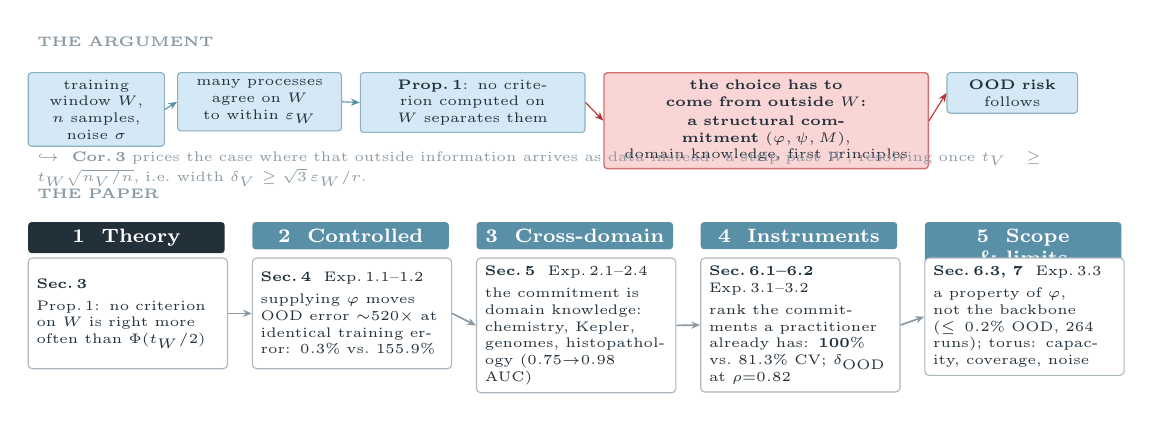
\begin{tikzpicture}[
  x=1pt,y=1pt,
  font=\scriptsize,
  >={Stealth[length=3.2pt,width=2.6pt]},
  arg/.style={draw=Btrain!70,fill=Ctrain,rounded corners=1.2pt,inner sep=2.6pt,
              align=center,text=Ink,font=\tiny},
  stage/.style={draw=Grey!70,fill=white,rounded corners=1.5pt,inner sep=3pt,
                align=left,text width=66pt,minimum height=40pt,anchor=north west,
                font=\tiny,text=Ink},
  head/.style={draw=none,fill=Btrain,text=white,rounded corners=1.2pt,
               inner sep=2.5pt,align=center,text width=66pt,anchor=north west,
               font=\scriptsize\bfseries},
  obj/.style={align=center,text=Bood,font=\tiny\itshape,text width=72pt,anchor=north west},
  thread/.style={draw=Csin!55!black,fill=Csin!12,rounded corners=1.5pt,inner sep=3pt,
                 align=center,text width=66pt,anchor=north west,font=\tiny,text=Ink},
  lbl/.style={text=Grey,font=\tiny\bfseries,anchor=west},
  aside/.style={align=left,text width=116pt,anchor=north west,font=\tiny,text=Grey},
]

% ===================== BAND 1 : THE ARGUMENT =====================
\node[lbl] at (0,127) {THE ARGUMENT};

\node[arg,anchor=north west,text width=44pt] (a1) at (0,116)
  {training window $W$,\\ $n$ samples, noise $\sigma$};
\node[arg,anchor=north west,text width=54pt] (a2) at (54,116)
  {many processes agree on $W$ to within $\varepsilon_W$};
\node[arg,anchor=north west,text width=76pt] (a3) at (120,116)
  {\textbf{Prop.\,1}: no criterion computed on $W$ separates them};
\node[arg,anchor=north west,text width=112pt,fill=Cood,draw=Bood!70,line width=0.5pt] (a4) at (208,116)
  {\textbf{the choice has to come from outside $W$:}\\[1pt]
   \textbf{a structural commitment} $(\varphi,\psi,M)$,\\ domain knowledge, first principles};
\node[arg,anchor=north west,text width=42pt] (a5) at (332,116)
  {\textbf{OOD risk} follows};

\draw[->,Btrain] (a1.east) -- (a2.west);
\draw[->,Btrain] (a2.east) -- (a3.west);
\draw[->,Bood]   (a3.east) -- (a4.west);
\draw[->,Bood]   (a4.east) -- (a5.west);

% subordinate: the data-side special case, deliberately not co-equal with the commitment.
% Full-width single line, clear of the a4 box (which bottoms out near y=94).
\node[aside,text width=396pt] (side) at (0,91)
  {$\hookrightarrow$\ \ \textbf{Cor.\,3} prices the case where that outside information arrives as
   data instead: a strip past $W$, resolving once $t_V\ge t_W\sqrt{n_V/n}$, i.e.\ width
   $\delta_V\ge\sqrt{3}\,\varepsilon_W/r$.};

% ===================== BAND 2 : THE PAPER =====================
\node[lbl] at (0,72) {THE PAPER};

% headers
\node[head,fill=Ink] at (  0,62) {1\ \ Theory};
\node[head] at ( 81,62) {2\ \ Controlled};
\node[head] at (162,62) {3\ \ Cross-domain};
\node[head] at (243,62) {4\ \ Instruments};
\node[head] at (324,62) {5\ \ Scope \& limits};

% bodies
\node[stage] (s1) at (  0,49)
  {\textbf{Sec.\,3}\\[2pt]
   Prop.\,1: no criterion on $W$ is right more often than $\Phi(t_W/2)$};
\node[stage] (s2) at ( 81,49)
  {\textbf{Sec.\,4}\ \ Exp.\,1.1--1.2\\[2pt]
   supplying $\varphi$ moves OOD error ${\sim}520\times$ at identical training error: $0.3\%$ vs.\ $155.9\%$};
\node[stage] (s3) at (162,49)
  {\textbf{Sec.\,5}\ \ Exp.\,2.1--2.4\\[2pt]
   the commitment is domain knowledge: chemistry, Kepler, genomes, histopathology ($0.75{\to}0.98$ AUC)};
\node[stage] (s4) at (243,49)
  {\textbf{Sec.\,6.1--6.2}\ \ Exp.\,3.1--3.2\\[2pt]
   rank the commitments a practitioner already has: $\mathbf{100\%}$ vs.\ $81.3\%$ CV; $\delta_{\mathrm{OOD}}$ at $\rho{=}0.82$};
\node[stage] (s5) at (324,49)
  {\textbf{Sec.\,6.3, 7}\ \ Exp.\,3.3\\[2pt]
   a property of $\varphi$, not the backbone ($\le0.2\%$ OOD, 264 runs); torus: capacity, coverage, noise};

\foreach \a/\b in {s1/s2,s2/s3,s3/s4,s4/s5}
  {\draw[->,Grey,semithick] (\a.east) -- (\b.west);}

\end{tikzpicture}
\end{document}
